\documentclass[a4j,12pt]{jreport}
%\documentclass{jreport}
\usepackage[dvipdfmx]{graphicx}
\usepackage[dvipdfmx]{graphics}
\usepackage{amsmath,amssymb}
% \usepackage{amsmath}
%\usepackage{pxjahyper}
\usepackage{here}
\usepackage{algorithm}
\usepackage{algpseudocode}
\usepackage{hhline} 
\usepackage[hang,small,bf]{caption}
\usepackage[subrefformat=parens]{subcaption}
\usepackage{url}
\captionsetup{compatibility=false}
\usepackage{bm}
\def\syaji{ \chapter*{謝辞} \addcontentsline{toc}{chapter}{謝辞}}
\renewcommand{\bibname}{参考文献}
\setlength{\textheight}{\paperheight}
\setlength{\topmargin}{4.6mm}
\addtolength{\topmargin}{-\headheight}
\addtolength{\topmargin}{-\headsep}
\addtolength{\topmargin}{-\headheight}
\addtolength{\textheight}{-60mm}

\setlength{\textwidth}{\paperwidth}
\setlength{\oddsidemargin}{-0.4mm}
\setlength{\evensidemargin}{-0.4mm}
\addtolength{\textwidth}{-50mm}

\begin{document}

%%%%%%%%%%%%%%%%%%%%%
% 表紙
%%%%%%%%%%%%%%%%%%%%%
\thispagestyle{empty}
\begin{center}
\begin{Large}
\vspace*{0.7cm}
{\large 卒業研究論文}\\
\vspace*{2.5cm}
{\bf 流体シミュレーションにおけるFLIP法の粒子半径の解析}\\
\vspace*{7.5cm}
須之内 俊樹\\
学籍番号\hspace*{1zw}19D8102020C\\
\vspace*{2.5cm}
中央大学理工学部情報工学科\hspace*{1zw} 形状情報処理研究室\\
\vspace*{3.0cm}
2023年3月\\
\end{Large}
\end{center}


%%%%%%%%%%%%%%%%%%%%%
% 概要
%%%%%%%%%%%%%%%%%%%%%
\newpage
\renewcommand{\baselinestretch}{1.25} \selectfont
\pagenumbering{roman}


\begin{center} {\large \bf{概 要}} \end{center}
流体シミュレーションとは,コンピュータを用いて,流体の運動を表現をする数理モデルの近似解を求めることである.
流体シミュレーションは,流体と触れる工業製品の開発や,コンピュータグラフィックスによる流体の表現に役立っている.コンピュータグラフィックスの分野では,流体の動きを忠実に再現することよりも,それらしい流体の運動を,計算負荷を抑えて計算することが重視されている.流体の種類や運動によって条件を設けることで,よりそれらしい動きをシミュレーションすることができる.例えば水は粘性の小さな,非圧縮性の流体であるため,流体の速度がさまざまな方向を向いているなら拡散し,シミュレーションの中で体積や密度が変化しないように振る舞うことが望ましい.
本研究では,水が重力に従って運動するシミュレーションにおいて,流体の動きがそれらしいかどうかについて,流体の体積の最大値と最小値を用いて,流体の体積の変動幅を計算し評価する.

シミュレーションの計算では,様々なパラメータが登場する.このパラメータはシミュレーションの手法や,表現したい流体,流体の運動の仕方によって,どの値が最も適切かは異なる.本研究では,流体の体積の変動幅の最小化するようなパラメータを解析する.

\vspace{1zw} \noindent
{\bf キーワード: }流体シミュレーション,数値流体力学,FLIP,非圧縮性条件

%%%%%%%%%%%%%%%%%%%%%
% 目次
%%%%%%%%%%%%%%%%%%%%%
\tableofcontents


\newpage
\pagenumbering{arabic}

%%%%%%%%%%%%%%%%%%%%%
% 1章
%%%%%%%%%%%%%%%%%%%%


%%%%%%%%%%%%%%%%%%%%%
% 2章
%%%%%%%%%%%%%%%%%%%%%
\chapter{序論} \label{chapter:2}

流体シミュレーションとは,コンピュータを用いて,流体の位置,速度,圧力などの物理量を計算するものである.ここでいう流体とは,空気,ガスなどの気体や,水,土砂の混ざった水,蜂蜜のような粘性がある液体,砂粒などの固体の粒など多岐にわたる.計算は流体力学の理論を元に,コンピュータを用いて計算できるように離散化しなければならない.流体力学の理論では,流体の静止状態を計算するものと,運動状態を計算するものに大きく分けることができる.また,2次元と3次元を扱うことができる.3次元では私たちの身の回りの現象を広くシミュレーションすることができる.2次元では,例えば,水面に広がる波紋や,異なる流体が作り出すマーブル模様などがシミュレーションできる.計算した結果を人間が見やすいように可視化することで,流体力学の理論だけでは把握することが困難な,空間に広がる流体の物理量の分布を把握することができるようになる.流体シミュレーションは,流体に触れる製品の設計・開発において,技術者が製品と流体の様子をシミュレーションして開発に役立てている.また,流体のアニメーションを作ることができるため,コンピュータグラフィックスの分野でも役に立っている.

計算機が登場する以前の流体力学は,実際の流体を用いて実験を繰り返さなければならなかったが,計算機が登場してからは,シミュレーションをすることで,計算機上で流体の振る舞いを確認できるようになった.計算機を使った流体力学を特別に,数値流体力学 (CFD: Computational Fluid Dynamics) と呼び分けることも多い.CFDは実験で得ることが困難な,流れ場全体の詳細な情報を得ることができる.CFDは流体に触れる製品の設計・開発に非常に大きな貢献をした.

また,コンピューターグラフィックスにおいても,流体のアニメーションを計算することができるCFDが貢献していて,映像作品やゲームなどで利用されている.コンピューターグラフィックスにおいては,それらしい流体の運動がリアルタイムでシミュレーションできることが重要視される.精度良く計算できることはそこまで重要視されておらず,場合によってはそれらしさのために,現実より大袈裟なシミュレーションをすることもある.
\chapter{非圧縮性流体のシミュレーション} \label{chapter:3}
\section{基礎概念}
数値流体力学では,シミュレーションする空間を離散化して計算を行う.離散化は,各辺が空間の座標軸に並行な計算格子を用いて空間を分割する.この計算格子上に物理量を定義して計算を行う.どのように定義して計算を行うかは手法によって異なる.ある時刻で空間の物理量の分布を計算した後,時刻を時間の刻み幅分進めて,次の時刻の計算をすることを繰り返してシミュレーションを行う.
\subsection{ナビエ・ストークス方程式} \label{subsec:nabie}
まず,この後に説明する流体シミュレーションの分野で一般的に使われている表記の説明をする.
\begin{quote}
	\begin{itemize}
		\item $\bm{x}:$ 流体の位置を表すベクトル.シミュレーションする空間によって2次元,または3次元になる.
		\item $t:$ 時刻を表す変数.シミュレーション開始の時刻を$0$とする.
		\item $\varDelta x,\varDelta t:$ 離散化する計算格子の格子幅,次の時刻までの時間幅.
		\item $\bm{u} (\bm{x},t) :$ 位置$\bm{x}$,時刻$t$での流体の速度ベクトル.
		\item $p (\bm{x},t) :$ 位置$\bm{x}$,時刻$t$での流体の圧力値.
		\item $\rho,\nu:$ それぞれ,流体の密度,流体の粘性.ここでは定数とする.
		\item $\bm{f}:$ 位置$\bm{x}$,時刻$t$での流体にかかる外力ベクトル.重力などはここに含める.シミュレーションの手法によっては外力を位置$\bm{x}$,時刻$t$によって変化する外力を扱うことができるが,今回は簡単のため,重力のみを扱い,どの位置でも,どの時刻でも一定の値として考える.
		\item $\nabla:$ 空間微分演算子ナブラ.スカラー場に作用させると勾配を表し,ベクトル場に作用させると発散を表す.3次元空間なので,$\nabla=  (\frac{\partial}{\partial x},\frac{\partial}{\partial y},\frac{\partial}{\partial z}) $ 
		\item $\frac{\rm{D}}{\rm{D}t} =\frac{\partial}{\partial t} + \bm{u} (\bm{x},t)  \boldsymbol{\cdot}\nabla$ :
		ラグランジュ微分,または物質微分.流体力学のような,連続体を扱う力学で用いられており,流れに沿って移動する物体と同じように移動する観測者から見た,物理量の時間変化率を表している.
	\end{itemize}
\end{quote}

下記の式 (\ref{eq:Navie}) で表される式を,ナビエ・ストークス方程式とよび,これは流体力学の支配方程式である.非線形二階微分方程式となっており,代数的に一般解を求める事ができない.下記の式 (\ref{eq:compressed}) は流体の圧縮性条件である.水や砂粒のように圧縮されない流体を扱うときは,流体の密度が常に一定,つまり密度の時間微分が0になり,それに伴い式 (\ref{eq:compressed}の左辺の第二項も0になる.これにより,式 (\ref{eq:uncompressed1}) と,式 (\ref{eq:uncompressed}) を得る.式 (\ref{eq:Navie}) と式 (\ref{eq:uncompressed}) または式 (\ref{eq:uncompressed1}) を連立することで非圧縮性流体の速度を求めることができる.ナビエ・ストークス方程式を扱う際は,コンピューターで近似解を解析的に求める手法が用いられる.
\begin{equation}\label{eq:Navie}
\frac{\partial}{\partial t}\bm{u} (\bm{x},t)  = - (\bm{u} (\bm{x},t)  \boldsymbol{\cdot}\nabla) \bm{u} (\bm{x},t)   - \frac{1}{\rho}\nabla p (\bm{x},t)  + \nu\nabla^2\bm{u} (\bm{x},t)  + \bm{f}
\end{equation}
\begin{equation}\label{eq:compressed}
\frac{\rm{D}}{\rm{Dt}}\rho + \nabla\boldsymbol{\cdot}\bm{u} (\bm{x},t)  = 0
\end{equation}
\begin{equation}\label{eq:uncompressed1}
\frac{\rm{D}}{\rm{Dt}}\rho  = 0
\end{equation}
\begin{equation}\label{eq:uncompressed}
\nabla\boldsymbol{\cdot}\bm{u} (\bm{x},t)  = 0
\end{equation}

式 (\ref{eq:Navie}) の右辺の第一項を移流項,第二項を圧力項,第三項を粘性項,第四項を外力項とよぶ.移流項は非線形項であり,その他は線形項である.

Losassoらが提案した,Marker And Cell法 (MAC法) \cite{MAC}と呼ばれる手法は,仮の速度$\bm{u}^*$を用いて,線形項を以下の式 (\ref{eq:linear}) ,非線形項を式 (\ref{eq:nonlinear}) のように分解して,段階的に計算する.
\begin{equation}\label{eq:linear}
\bm{u} (\bm{x},t+1)  =  \bm{u}^* - \varDelta t (\frac{1}{\rho}\nabla p (\bm{x},t)  + \nu\nabla^2\bm{u} (\bm{x},t)  + \bm{f}) 
\end{equation} 

\begin{equation}\label{eq:nonlinear}
\bm{u}^* = \bm{u} (\bm{x},t)  - \varDelta t (\bm{u} (\bm{x},t)  \boldsymbol{\cdot}\nabla) \bm{u} (\bm{x},t)  
\end{equation}

ナビエ・ストークス方程式を離散化する方法は,大きく分けて格子法と粒子法がある.

\subsection{格子法} \label{subsec:grid}
格子法とは,流体を扱う空間を正方形や立方体の格子に区切り,格子の中心や辺,頂点などに物理量を配置して計算する方法である.区切る格子の数が多いほど,流体の詳細な動きが計算できるが,計算負荷は増加する.格子法は,規則正しく並んだ格子で空間を離散化することで,微分演算を差分法などの方法で近似することができ,実装しやすい.

微分計算の差分近似によって,無視されてしまう項が存在する.格子法での移流項の計算に用いられる差分近似で無視される項を,数値拡散,または人工粘性と呼ぶ.格子法での移流項の計算には風上差分がよく用いられるが,簡単のため,前進差分を用いる.格子法の欠点は,この数値拡散が決して小さくないため,移流項の精度があまりよくないことである.しかし,以下の移流項の計算によって,移流項の数値拡散として粘性項に似た形の式が現れる.従って,粘性項は移流項の数値拡散として扱い,まとめて計算されることが多い.また,水飛沫などの,液体が細かく分散するような計算は困難である.これは,微分の計算を差分で近似することで,隣接する格子との相互関係を用いて計算することになるため,液体が分散すると計算がうまくいかないためである.

\subsubsection{格子法における移流項の計算} \label{subsec:gridadvect}
\begin{equation}\label{eq:uncalculated_pressure_before}
\frac{\partial}{\partial t}\bm{u} (\bm{x},t)  = -\bm{u} (\bm{x},t) \frac{\partial}{\partial \bm{x}}\bm{u} (\bm{x},t)
\end{equation} 

偏微分演算子を前進差分$\frac{\partial}{\partial \bm{x}}\bm{u} (\bm{x},t)  = \frac{\bm{u} (\bm{x}+\varDelta \bm{x},t)  - \bm{u} (\bm{x},t) }{\varDelta \bm{x}}$を用いて離散化すると,
$$\frac{\partial}{\partial t}\bm{u} (\bm{x},t)  =  -\bm{u} (\bm{x},t) \frac{\bm{u} (\bm{x}+\varDelta \bm{x},t)  - \bm{u} (\bm{x},t) }{\varDelta \bm{x}}$$
が得られる.
二変数のテーラー展開$f (a+h,b+k)  \fallingdotseq \sum\limits_{t=0}^n \frac{1}{t!} (h\frac{\partial}{\partial \bm{x}} + k\frac{\partial}{\partial y}) ^t f (a,b) $を二次まで行い,式を整理すると,
$$\frac{\partial}{\partial t}\bm{u} (\bm{x},t)  = -\frac{1}{2!\varDelta \bm{x}}\bm{u} (\bm{x},t) \left (  (\bm{u} (\bm{x},t) +\varDelta t\frac{\partial}{\partial \bm{x}}\bm{u} (\bm{x},t)  +  (\varDelta \bm{x}) ^2\frac{\partial^2}{\partial \bm{x}^2}\bm{u} (\bm{x},t)  \right) $$
            
$$\frac{\partial}{\partial t}\bm{u} (\bm{x},t)  =  -\bm{u} (\bm{x},t) \left (\frac{\partial}{\partial \bm{x}}\bm{u} (\bm{x},t)  + \varDelta \bm{x}\frac{\partial^2}{\partial \bm{x}^2}\bm{u} (\bm{x},t)  \right) $$

$$ \frac{\partial}{\partial t}\bm{u} (\bm{x},t)  =  -\bm{u} (\bm{x},t) \frac{\partial}{\partial \bm{x}}\bm{u} (\bm{x},t)  -\bm{u} (\bm{x},t) \varDelta \bm{x}\frac{\partial^2}{\partial \bm{x}^2}\bm{u} (\bm{x},t) $$

が得られる.ここで,$ -\bm{u} (\bm{x},t) \varDelta \bm{x} = \mu$とし,$\frac{\partial^2}{\partial \bm{x}^2}\bm{u} (\bm{x},t)  = \nabla^2\bm{u} (\bm{x},t) $とすれば,
\begin{equation}\label{eq:uncalculated_pressure_after}
\frac{\partial}{\partial t}\bm{u} (\bm{x},t)  =  -\bm{u} (\bm{x},t) \frac{\partial}{\partial \bm{x}}\bm{u} (\bm{x},t)  +\mu\nabla^2\bm{u} (\bm{x},t) ) 
\end{equation} 
が得られる.式( \ref{eq:uncalculated_pressure_before}) と式( \ref{eq:uncalculated_pressure_before}) を比較すると,右辺の二項目が数値拡散であること,そして数値拡散は粘性項の式とよく似ていることがわかる.
\subsubsection{格子法における非線形項の計算} \label{subsec:gridpressure}
式 (\ref{eq:linear}) の粘性項は先述の通り省略し,外力項は事前に流速に与えて扱うことができるため省略する.残った圧力項の計算について考える.ただし,移流項を先に計算し,$\bm{u}^*$は既知のものとする.
\begin{equation}\label{eq:uncalculated_pressure}
\bm{u} (\bm{x},t+1)  =  \bm{u}^* - \frac{\varDelta t}{\rho}\nabla p (\bm{x},t) 
\end{equation} 
両辺の発散をとると,
$$\nabla\boldsymbol{\cdot}\bm{u} (\bm{x},t+1)  =  \nabla\boldsymbol{\cdot}\bm{u}^* - \frac{\varDelta t}{\rho}\nabla^2 p (\bm{x},t) $$
が得られ,流体の非圧縮性条件,$\nabla\boldsymbol{\cdot}\bm{u} (\bm{x},t)  = 0$により,左辺は0になるため,
\begin{equation}\label{eq:calculated_pressure}
\nabla\boldsymbol{\cdot}\bm{u}^* = \frac{\varDelta t}{\rho}\nabla^2 p (\bm{x},t) 
\end{equation} 
が得られる.この式を満たすような圧力を求め,上記の式 (\ref{eq:uncalculated_pressure}) に代入することによって,次の時刻の流速$\bm{u} (\bm{x},t+1) $が計算できる.式 (\ref{eq:calculated_pressure}) のような微分方程式はポアソン方程式と呼ばれ,境界条件として,扱う領域の境界での$p (\bm{x},t) $の値を計算前に定めることで,式を満たすような変数を求めることができる.
\subsubsection{格子法における物理量の位置の定義方法} \label{subsec:grid_sampling}
\begin{figure}[htbp]
\begin{center}
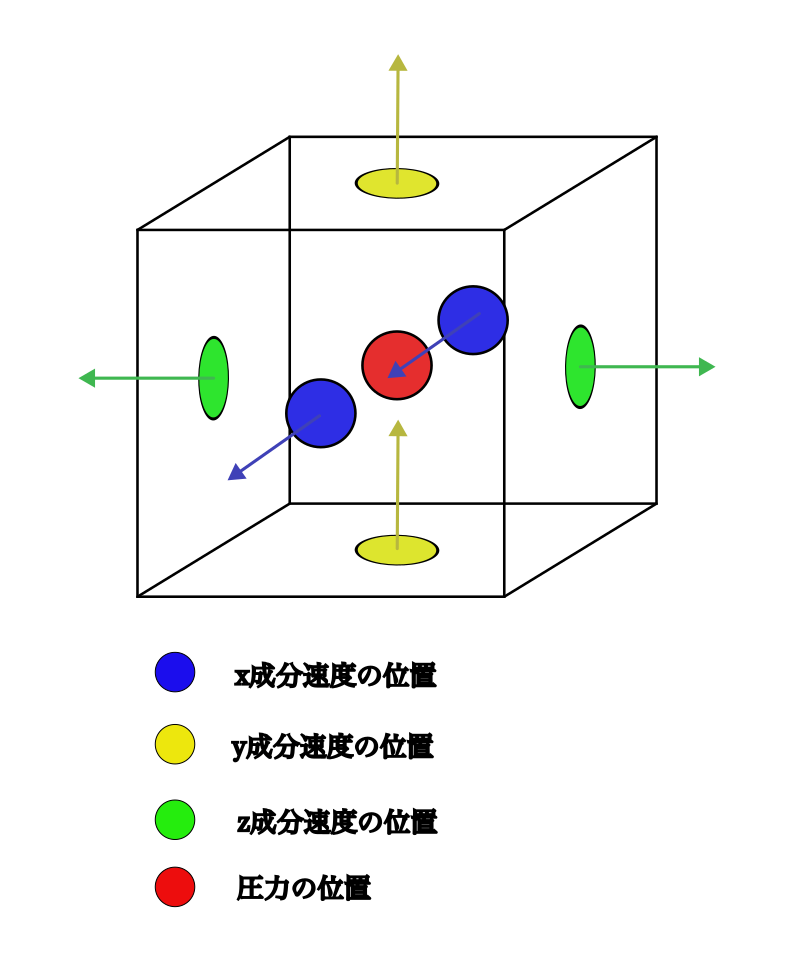
\includegraphics[width=80mm]{3dstaggerd.png}
\caption{スタッガード格子}
\label{fig:staggerd}
\end{center}
\end{figure}

CGの流体シミュレーションにおいて,MAC法\cite{MAC}で格子を離散化する方法がよく用いられている.この手法では,扱う領域を正方形や立方体の格子に区切って,その格子状に物理量を定義する.下記の図\ref{fig:staggerd}のように,格子の中心を圧力の位置に定義し,格子面の中心に,その格子面と垂直な流速の成分の位置を定義する.例えば$xy$平面に並行な格子面には,その地点での流速の$z$成分を配置する.これはスタッガード格子と呼ばれている.この手法は格子点に全ての物理量を配置するコロケート格子と比べ,境界付近の流速が表現しやすく,それらしいシミュレーションができるだけでなく,ポアソン方程式の境界条件の設定も容易である.具体的には,格子が壁に隣接している場合,その面からの流体の流入出はゼロであるため,壁面方向の圧力差と,壁面と隣接している面の中心に配置されている流速成分は共にゼロにする.

\subsubsection{スタッガード格子を用いた,格子法の線形項の計算の離散化方法}
\begin{figure}[htbp]
\begin{center}
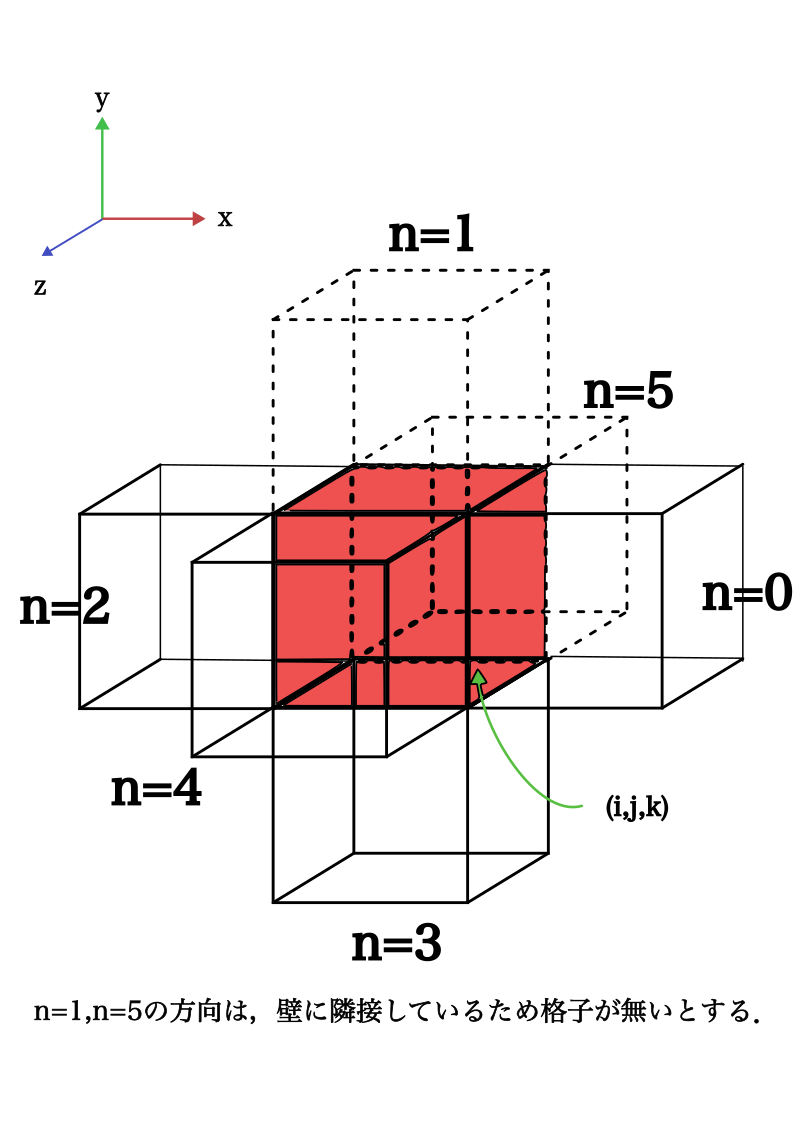
\includegraphics[width=80mm]{pressure_model.png}
\caption{圧力計算のモデル}
\label{fig:pressure_model}
\end{center}
\end{figure}
圧力項の計算を,スタッガード格子を用いて離散化するため,先ほどの式 (\ref{eq:calculated_pressure}) を考える.
$$\nabla\boldsymbol{\cdot}\bm{u}^* = \frac{\varDelta t}{\rho}\nabla^2 p (\bm{x},t) $$
スタッガード格子では圧力と流速が配置してある位置がずれている.従って,空間微分に対して同じ差分を適用すると,同じ幅で差分を取ったとしても離散化される空間の位置がずれてしまうため,空間微分に対して同じ差分は適応できない.そこで差分を取るのではなく,両辺をセルの領域で積分して考える.
$$\int_V\nabla\boldsymbol{\cdot}\bm{u}^* dV= \int_V\frac{\varDelta t}{\rho}\nabla^2 p (\bm{x},t) dV$$
両辺にガウスの発散定理を適用すると,周回積分の形で表せる.
$$\oint_V\bm{u}^*\boldsymbol{\cdot}\bm{n} dV= \oint_V\frac{\varDelta t}{\rho}\nabla p (\bm{x},t) \boldsymbol{\cdot}\bm{n}dV$$
この式はスタッガード格子において,周回積分は格子の各面で境界条件を考えて,全ての面の物理量を足すことで表すことができる.
ここで離散化のため,$x軸方向にi番目,y軸方向にj番目,z軸方向にk番目の格子をg_{i,j,k},g_{i,j,k}の圧力をp_{i,j,k}と定義し,$図\ref{fig:pressure_model}のようなモデルを考える.

まず,整数$n=0,1,2,\cdots 5$までを,それぞれ格子の各面の方向に割り振る.図\ref{fig:pressure_model}の場合,$n=0$は$x$軸正の方向,$n=1$は$y$軸正の方向,$n=2$は$x$軸負の方向,$n=3$は$y$軸負の方向,$n=4$は$z$軸正の方向,$n=5$は$z$軸負の方向に割り振る.ここで,この整数$n$を使って,いくつかの配列や変数を定義する.
\begin{quote}
	\begin{itemize}
		\item $F_n$ 格子の面の各方向に隣接しているものが流体なら$1$,壁面なら$0$を取るブーリアン値.
		
		図\ref{fig:pressure_model}の場合,$n=0$に対応する$x$軸正の方向と,$n=5$に対応する$z$軸負の方向は壁に隣接していて格子がないため,$F_0,F_5 = 0,F_1,F_2,F_3,F_4 = 1$となる.
		\item $D_n$ 格子の面の各方向に垂直で,格子の外側を向く単位ベクトルを表す係数.向いている方向が座標軸の正の向きなら+1,					負の向きなら$-1$を取る整数値.
		
		図\ref{fig:pressure_model}の場合,座標軸の正の方向に向いているのは$n=0,n=1,n=4$に対応する方向で,それ以外は負の方向に向いているため,
		$F_0,F_1,F_4 = 1,F_2,F_3,F_4 = -1$となる.
		\item $p_n$ 割り振られた方向に隣り合っている格子の圧力値.
		図\ref{fig:pressure_model}の場合,$p_0 = p_{i+1,j,k}$,$p_1 = p_{i,j+1,k}$,$p_2 = p_{i-1,j,k}$,$p_3 = p_{i,j-1,k}$,$p_4 = p_{i,j,k+1}$,$p_5 = p_{i,j,k-1}$となるが,境界条件を考えると,壁に隣接している格子との圧力値の勾配を$0$にするため,$p_0 = p_{i,j,k}$,$p_5 = p_{i,j,k}$である.
		\item $\nabla\bm{p_n}$ 割り振られた方向の圧力勾配.前方差分によって,$\nabla \bm{p_n} (\bm{x},t)  = \frac{p_n - p_{i,j,k}}{\varDelta x}$と近似できる.
		\item $u_n$ $g_{i,j,k}$に配置されている流速値で,割り振られた方向の格子面に配置されている流速値.壁に隣接している方向は流速を$0$にするため,$u_0 = 0$,$u_5 = 0$である.
	\end{itemize}
\end{quote}

定義した配列や変数を用いて,周回積分の形で表された式を離散化することで,
$$ \sum_{n}\bm{u_n}^*D_nF_n\varDelta x = \sum_{n}\frac{\varDelta t}{\rho}\nabla p_n (\bm{x},t) F_n\varDelta x $$
が得られ,圧力勾配を$\nabla p_n (\bm{x},t)  = \frac{p_n - p_{i,j,k}}{\varDelta x}$で近似すると,

$$ \sum_{n}\bm{u_n}^*D_nF_n\varDelta x = \sum_{n}\frac{\varDelta t}{\rho}\frac{p_n (\bm{x},t) - p_{i,j,k} (\bm{x},t) }{\varDelta \bm{x}}F_n\varDelta x $$
が得られる.この式を整理すると,
\begin{equation}\label{eq:discretized_pressure}
\sum_{n}\bm{u_n}^*D_nF_n= \sum_{n}\frac{\varDelta t}{\rho}\frac{p_n (\bm{x},t)  - p_{i,j,k} (\bm{x},t) }{\varDelta \bm{x}}F_n
\end{equation} 
が得られる.
式 (\ref{eq:discretized_pressure}) は$p$についての連立一次方程式となっている.全ての格子に対して式 (\ref{eq:discretized_pressure}) を考えることになるため,連立方程式は規模が大きくなる.従って,直接法ではなく反復法を用いて,必要な精度で計算を打ち切って計算する.連立方程式の解法としては,前処理付き共役勾配法がよく用いられている.

\subsubsection{ディリクレ境界条件} \label{subsec:Dirichlet}
圧力項の計算を離散化した式 (\ref{eq:discretized_pressure}) は,求めたい圧力分布の式 (\ref{eq:uncalculated_pressure}) を満たすような解が得られるが,得られた解がシミュレーション内で,良い圧力として振る舞うかどうかは考えなければならない.ディリクレ境界条件は,扱う領域を流体と気体の領域に分割し,流体の物理量のみを考える際に用いる境界条件で,流体が存在しない格子の圧力値を$0$とする.ディリクレ境界条件を考えずに流体の圧力のみを計算すると,気体の領域とされている場所にも流体の圧力が計算できてしまう.そのため,気体と液体の領域に分割するようなシミュレーションで,気体の圧力が液体の圧力に及ぼす影響が小さい場合は,圧力にディリクレ境界条件を追加した方が,より良い圧力分布になると言える.

\subsection{粒子法} \label{subsec:particle}
粒子法とは,流体をいくつかの小さな粒子の集まりとして考え,各粒子に物理量を与えて計算をする方法である.本来は流体は,アボガドロ数 ($N_A = 6.02*10^{23}$) 単位の分子が動いているが,これら全てを計算機で扱うのは現実的でないため,いくつかの分子の動きを一つの粒子にまとめて扱う.粒子の数が多いほど実際の現象に近づき,精度が良くなるが,計算負荷は増加する.利点として,以下の計算によって,移流項の計算に数値拡散が発生しないことが確認できるため,移流項が精度良く計算できる.また,格子法では水飛沫の表現が困難であるが,粒子法は粒子が存在する場所に液体が存在すると考えるため,粒が飛び散りさへすれば水飛沫のような表現になる.欠点として,粒子が飛び散ったときに粒子の影響範囲内に他の粒子がいないとき,計算がうまくできないことから,正確な物理量の分布が計算できる訳ではない.また,対象の流体以外は計算しないことが多いため,例えば水と空気が入り混じるようなシミュレーションを考える際,水の計算のみをすることで,空気の影響が無視されてしまう.
\subsubsection{粒子法における移流項の計算} \label{subsec:particleadvect}
簡単のため,ナビエストークス方程式から粘性項と外力項を取り除いた,オイラー方程式と呼ばれるものについて考える.
$$\frac{\partial}{\partial t}\bm{u} (\bm{x},t)  = - (\bm{u} (\bm{x},t) \boldsymbol{\cdot}\nabla) \bm{u} (\bm{x},t)  - \frac{1}{\rho}\nabla \bm{p}$$
粒子法はラグランジュ微分を用いることで、移流項の計算が単純になる。
時刻$t_0$に位置$\bm{x_0}$にある流体の速度を$\bm{u} (\bm{x_0},t_0) $とする.$\varDelta t$秒後の位置は$\bm{x_0}+v (\bm{x_0},t_0) \varDelta t$になっているので,時刻$t_0+\varDelta t$の流体の速度は、$\bm{u} (\bm{x_0}+\bm{u} (\bm{x_0},t_0) \varDelta t,t_0+\varDelta t) $となる。この間の速度変化$\varDelta \bm{u}$をテイラー展開を用いて表すと,

$$ \varDelta \bm{u} = \bm{u} (\bm{x_0}+v\varDelta t,t_0+\varDelta t)  - \bm{u} (\bm{x_0},t_0)  = \frac{\partial \bm{u} (\bm{x_0},t_0) }{\partial \bm{x}}\bm{u} (\bm{x_0},t_0) \varDelta t + \frac{\partial \bm{u} (\bm{x_0},t_0) }{\partial t}\varDelta t$$

両辺を$\varDelta t$で割ると,
$$ \frac{\varDelta \bm{u}}{\varDelta t} = \frac{\partial \bm{u} (\bm{x_0},t_0) }{\partial \bm{x}}\bm{u} (\bm{x_0},t_0)  + \frac{\partial \bm{u} (\bm{x_0},t_0) }{\partial t}$$
$$ \frac{\varDelta \bm{u}}{\varDelta t} =  (\bm{u}\boldsymbol{\cdot}\nabla) \bm{u} + \frac{\partial \bm{u} (\bm{x_0},t_0) }{\partial t}$$

ラグランジュ微分,つまり,粒子を流れに沿って動かしたときの変化量が,オイラー方程式の移流項になっている.粒子法では,物理量をもった粒子自体を動かすだけで,移流項の計算をすることができる.

\subsubsection{粒子の位置の補正} \label{subsec:fixparticlepos}
粒子を流速に沿って移動させた際,境界をすり抜けてしまうことがある.この対策として,各時刻で,飛び出してしまった粒子を境界内に戻す手法がある.戻す方向や距離は,等値面を使って比較的簡単に計算することができる.シミュレーションの境界を等値面で表したものを,レベルセットサーフェスと呼ぶこともある.

粒子法で流体の非圧縮性条件を満たすようなシミュレーションをするには,大きく分けて二つの方法がある.1つはポアソン方程式を解く方法である.安本らのMPS法\cite{MPS}などの粒子法は,格子法でも登場したポアソン方程式を解く方法を取っているが,離散化が格子法のように簡単には行えず,精度や計算時間に問題がある.二つ目は,粒子の密度を計算し,密度が一定になるように粒子を移動させたり,粒子を増減させる方法である.Lucyらの\cite{SPH}SPH法などはこのような方法をとっている.この方法はナビエストークス方程式の計算過程とは関係ないため,粒子の分布の変化に伴って粒子の物理量も補正する必要がある.一つ目の方法は流体の非圧縮性条件として,式 (\ref{eq:uncompressed}) を用いているのに対し,二つ目の方法は,式 (\ref{eq:uncompressed1}) を使っていると考えることもできる.式 (\ref{eq:uncompressed1}) を利用する手法は確実に密度が保存されるため,密度に関しては頑健であるのに対し,圧力が振動してしまう.それに対し式 (\ref{eq:uncompressed}) を用いる方法は密度の計算誤差が蓄積していってしまうのに対し,圧力の振動を防ぐことができる.

\section{関連研究} \label{sec:reratedworks}
\subsection{PIC (Particle In Cell) } \label{subsec:PIC}
粒子法は移流項の計算の精度がよく,他の線形項の精度が悪い.格子法は移流項の精度が悪く,他の線形項の精度が良い.Harlowらの手法Particle In Cell (PIC) 法\cite{PIC}は,粒子法と格子法の利点を組み合わせた手法である.粒子と格子の間で物理量を受け渡し,移流項の計算を粒子で行い,その他の計算を格子で行う.
この分野でよく使用される表記の説明をする.

流速などの物理量は,粒子が持っているのか,格子が持っているのか区別する必要があり,また,その時刻によって異なるため,上付き文字として時刻を,下付き文字として物理量を持っているのが粒子なのか格子なのかを表記する.例えば
時刻$t$において,格子の物理量が格納されている位置を$\bm{x}^t_i =  (x^t_i,y^t_i,z^t_i) $,粒子の位置を$\bm{x}^t_p =  (x^t_p,y^t_p,z^t_p) $,格子の流速を$\bm{v}^t_i$,粒子の流速を$\bm{v}^t_p$,格子の質量を$m^t_i$,粒子の質量を$m^t_p$とする.ただし,基本的には粒子の質量は時刻によらず一定である.また,格子の中に入っている粒子についての物理量は,$v_{ip}$のように$iとp$を両方つけて表記する.
\subsubsection{粒子と格子での物理量の受け渡し} \label{subsec:P2GG2P}
また,格子の一辺の長さを$h$とする.まず,格子と粒子の位置による重みを以下のように定義する.
\begin{equation}\label{eq:weight}
w^t_{ip} = N^t_i (\bm{x}^t_p)  = N (\frac{1}{h} (x^t_p - x^t_i) ) \boldsymbol{\cdot}N (\frac{1}{h} (y^t_p - y^t_i) ) \boldsymbol{\cdot}N (\frac{1}{h} (z^t_p - z^t_i) ) 
\end{equation} 

$N (x) $はカーネル関数であり,以下のように定義する.
\begin{equation}\label{eq:kernel}
N (x)  = 
\begin{cases}
\frac{1}{2}|x|^3 - |x|^2 + \frac{2}{3} &  (0\leqq|x|<1),  \\
\frac{1}{6} (2-|x|) ^3 &  (1\leqq|x|\leqq2),  \\
0 & \rm{else}.
\end{cases}
\end{equation} 
カーネル関数の関数値は,引数の絶対値が0に近いほど大きく,絶対値が大きくなるに従って小さくなっていく,微分可能な関数である.粒子と格子の距離が格子の幅の二倍以上離れていると重みは0になるため,その範囲内の粒子についてのみ考えればよい.

次に格子の質量について,以下のように定義する.
\begin{equation}\label{eq:grid_m}
m^t_i = \sum\limits_p m^t_pw^t_{ip}
\end{equation} 

式 (\ref{eq:grid_m}) を使って,粒子の速度を格子の速度に以下のように受け渡す.

\begin{equation}\label{eq:P2G}
\bm{v}^t_i = \sum\limits_p w^t_{ip}\bm{v}^t_p / m^t_i
\end{equation} 

式 (\ref{eq:P2G}) は,両辺に$m^t_i$をかけることで運動量についての式になり,シミュレーション全体では運動量が保存しているように振る舞う.

\subsubsection{PICのアルゴリズム} \label{subsec:PIC_algo}
PICの大まかなアルゴリズムは以下のようになる.
\begin{quote}
	\begin{itemize}
		\item 粒子の流速$\bm{v}^{t}_p$を式 (\ref{eq:P2G}) に従って,格子の流速$\bm{u} (\bm{x},t) $に受け渡す.
		\item 格子の流速に重力等の外力の情報を反映させる.例えば重力は$\bm{u} (\bm{x},t)  += \bm{f}\varDelta t$のように反映させる.
		\item \ref{subsec:gridpressure}のように,格子法と同じ方法で格子の圧力項を計算する.ここで,格子の次の時刻での流速$\bm{u}_t (\bm{x},t+1) $が求められる.
		\item 格子の次の時刻での流速$\bm{u} (\bm{x},t+1) $を粒子に受け渡し,粒子の次の時刻の流速$p\bm{v}_{t+1}$を求める.この際も式 (\ref{eq:P2G}) と同様の重みを使用する.
		\item 粒子の位置を$\bm{v}^{t+1}_p$を使って,$\bm{x}^{t+1}_p = \bm{v}^{t+1}_p\varDelta t $のように更新する.
	\end{itemize}
\end{quote}

一般的に粒子の数が格子の数よりも多いため,粒子から格子に物理量を受け渡す際に,一つの格子に対して複数の粒子が対応する.この際に,粒子法と比べると粒子の粘性が高くなるような効果がある.これを人工粘性と呼ぶ.格子法とは異なり,移流項を計算すると粘性項を別途計算する必要があるが,PICは人工粘性があるため,粘性項は計算しなくとも粘性を表現できる.しかし,意図しない粘性が含まれてしまうため,粘性の小さな流体のシミュレーションには不向きである.この人工粘性を解決するためのさまざまな手法が提案されている.
\subsection{FLIP (Fluid Implicit Particles) } \label{subsec:FLIP}
BrackbillらはPICのアルゴリズムを少し変更した,Fluid Implicit Particles (FLIP) 法\cite{FLIP}を提案した.FLIPは格子の速度を粒子の速度に渡す際,格子の速度をそのまま渡すのではなく,格子の速度の変化分を粒子に受け渡す.アルゴリズム内では,線形項の計算に入る前に現在の流速を保存しておき,圧力項の計算が終わってから,格子の速度を粒子の速度に受け渡す際に,粒子の速度を直接計算するのでなく,変化分を重みづけして計算し,現在の粒子の速度に加算する.PICは格子の影響の範囲内にある粒子の速度が同じような方向に向いてしまうことあるが,速度の変化分を計算することで,この問題がなくなり,PICの人工粘性を解消することができる.問題点として,数値誤差が蓄積し続ける,粒子の勢いがほとんど減衰しないなどがある.実際の流体は粘性が少なからずあるため,粘性を別で考える必要がある.
\subsection{PIC/FLIP} \label{subsec:PIC/FLIP}
FLIPの粘性を考える際,PICで計算した速度の影響を少しだけ入れることで,人工粘性を持たせる方法である.PICで計算した速度を$\bm{v}_{\rm{PIC}}$,FLIPで計算した速度を$\bm{v}_{\rm{FLIP}}$とすると,PIC/FLIPの速度$\bm{v}_{\rm{PF}}$ は以下のように計算する.

\begin{equation}\label{eq:PIC/FLIP}
\bm{v}_{\rm{PF}} =\alpha \bm{v}_{\rm{FLIP}} + (1-\alpha)  \bm{v}_{\rm{PIC}}
\end{equation} 

ここで$\alpha$は$0$から$1$までの係数で,小さくするほどPICの速度の割合が大きくなり,粘性が大きくなる.
しかし,FLIPの数値誤差が蓄積する問題は解決できず,PICの角運動量や運動エネルギーが失われてく問題も残る.

\subsection{発展手法} \label{subsec:APIC/ASFLIP}
\subsubsection{APIC} \label{subsec:APIC}
PICやFLIPに残る問題点を解決するため,それらを発展させた手法が多く生み出されてきている.岩間らのAffine Particle-In-Cell (APIC) 法\cite{APIC}は,各粒子について,粒子の運動エネルギーや角運動量を保存するための行列を別途用意し,粒子の速度にかけることでPICの角運動量や運動エネルギーが失われてく問題を解消している.PICの粘性が大きくなってしまう問題もある程度対応でき,FLIPを混ぜなくとも良くなるため,FLIPの問題点を抱えずに済んでいる.しかし,粘性が大きくなる問題に完全には対応できていないため,PIC/FLIPよりも常に優れているというわけではない.粘性の小さな流体が,激しく流体が運動するようなシミュレーションはPIC/FLIPの方が適している.

\subsubsection{PIC/FLIPの粒子位置の修正}\label{subsubsec:fixparticlepos}
節\ref{subsec:fixparticlepos}で粒子法における
$\frac{\rm{D}}{\rm{Dt}}\rho  = 0$や,
$\nabla\boldsymbol{\cdot}\bm{u} (\bm{x},t)  = 0$を満たすように,
粒子位置の修正法を紹介したが,PIC/FLIPは圧力項を粒子法で計算しないため,ポアソン方程式を解く方法を使用するのは手間がかかる.そのため,式 (\ref{eq:uncompressed1}) のように,密度が一定になるように直接補正する方法を紹介する.まず,全ての粒子について,粒子の密度分布を修正する方向ベクトル$\varDelta p_i$を計算する.
\begin{equation}\label{eq:w_smooth}
W_{\rm{smooth}} (\bm{r},h)  = \rm{max} (0,1-||r||^2/h^2) 
\end{equation} 

\begin{equation}\label{eq:w_sharp}
W_{\rm{sharp}} (\bm{r},h)  = \rm{max} (0,h^2/||r||^2 - 1) 
\end{equation} 

\begin{equation}\label{eq:fixVector}
\varDelta p_i = -\gamma \varDelta td_i\sum\limits_j \frac{p_j - p_i}{||p_j - p_i||}W_{\rm{smooth}} (p_j - p_i,d_i) 
\end{equation} 

ここで,$W_{\rm{smooth}}$は平滑化カーネルで,$W_{\rm{sharp}}$は中心で値が無限大になるようなカーネル関数である,$\gamma$は修正度合いを表す係数で,$d_i$は粒子半径である.$p_i$,$p_j$は粒子の位置である.このベクトルに従って粒子の位置を$x_p += \varDelta p_i$のように修正する.次に,粒子の物理量をそのままに,粒子の位置を修正すると,粒子によって表現されている流体の物理量の分布が歪んでしまうため,粒子の物理量も計算し直す必要がある.粒子$i$の物理量$q (\bm{p_i}) $ は以下のように修正する.
\begin{equation}\label{eq:fixVelocity}
q (\bm{p_i})  = \frac{\sum\limits_j m_jq_jW_{\rm{sharp}} (p^*_j - p_i,d_i) }{\sum\limits_j m_jW_{\rm{sharp}} (p^*_j - p_i,d_i) }
\end{equation} 

ここで,$q_j,m_j,p^*$はそれぞれ,粒子の物理量,粒子の質量,修正前の粒子の位置である.この手法による粒子位置の修正は,PICのように角運動量や運動エネルギーが失われてく性質があるため,視覚的には人工粘性が大きくなるような効果がある.この手法は,一度の移動で密度が完全に保存するように移動させるわけではなく,粒子密度が大きい空間にいる粒子が,密度が小さい空間に移動することによって密度が高くなるのを防ぐものである.

\subsection{MPS法における不自然な数値振動の抑制}\label{subsec:japan}
\ref{subsec:fixparticlepos}で述べたように,流体の非圧縮性条件に従った粒子位置の修正方法には種類があり,それぞれ利点と欠点がある.PICは格子法と粒子法を混ぜ合わせて計算する手法であり,PIC/FLIPはPICとFLIPを混ぜ合わせて計算する手法であるように,近藤らは,流体の非圧縮性条件を満たすための手法を混ぜ合わせる手法\cite{kondou}を提案した.圧力振動と密度をよく保存することは一得一失の関係であり,それぞれに特化した手法を混ぜ合わせることで,既存の他の手法よりも安定した計算と,なめらかな圧力分布を実現している.

\chapter{提案手法} \label{chapter:4}
\section{FLIPの実装} \label{sec:ImpFLIP}
本研究では,式 (\ref{subsubsec:fixparticlepos}) を用いて,流体の非圧縮性を満たすように粒子位置を修正する.その際,視覚的には人工粘性が大きくなるような効果があるため,PIC/FLIPのようにPICで計算した速度を少し混ぜることはせず,FLIPの速度のみを用いる.本手法では3次元の行列や,サイズの大きい行列やベクトルを扱うため,C++の線形代数ライブラリ,Eigenを用いる.また,Eigenの連立方程式のソルバーを用いて,ポアソン方程式を解くことができる.
スタッガード格子の$x$方向の数を$N_x$または\texttt{Nx},$y$方向の数を$N_y$もしくは\texttt{Ny},$z$方向の数を$N_z$もしくは\texttt{Nz}とすると,スタッガード格子は水平方向の速度,鉛直方向の速度,圧力を3次元配列に保存することで実装できる.ぞれぞれの配列のコード内での定義は以下のようになる.
\begin{quote}
	\begin{itemize}
		\item $x$方向の速度 \texttt{double vx[Nx+1][Ny][Nz]} 
		\item $y方向の速度 \texttt{double vy[Nx][Ny+1][Nz]}$ 
		\item $z方向の速度 \texttt{double vz[Nx][Ny][Nz+1]}$ 
		\item $圧力 \texttt{double p[Nx][Ny][Nz]}$
	\end{itemize}
\end{quote}
粒子から格子に速度を受け渡す際や,外力の影響を考える際に,格子の質量が必要である.この質量は,水平方向と鉛直方向それぞれの速度がサンプリングされている位置と同じ位置に配置する.また,外力は質量と同じ位置での圧力値を2次元配列で与えるが,重力のような保存力を考える場合,格子にかかる力は格子の質量によって異なるため,加速度のみを2次元配列で与え,必要に応じて重力を乗算する.また,後にFLIPで流速の変化量を計算するために,変化前の流速を保存する配列を同時に用意する.
粒子については,一つの粒子を,粒子の位置,速度,PICで計算した速度,FLIPで計算した速度をメンバ変数にもつ構造体で実装し,その構造体の配列で全粒子を管理する.
粒子は,実装するシミュレーションの次元を$d$とすると,一つの格子に$2^d$個配置することが多い.つまり,粒子数は2次元の場合だと$4N_xN_y$となる.ここまでをシミュレーションの前に初期化する.

粒子-格子での物理量の受け渡しの際に,格子のサンプリング点の周辺にある粒子を探索する必要がある.粒子の位置を,格子の数と格子の一辺の長さをかけた数で割ることで,粒子がどの格子の近くにあるか判定することができるが,ナイーヴに格子ごとに近傍の粒子を探索
して実装すると,計算量が大きくなってしまう.この問題は,格子ごとにどの粒子が入っているのかを保存するようなデータ構造を,各タイムステップで更新することで解決できる.各タイムステップの最後で粒子の位置を移動させるため,各タイムステップの最初でこのデータ構造を更新する.本手法ではstructured gridを使用している.c++ではハッシュテーブルクラス,\texttt{unordered\_map}のキーを格子の位置,値を格子に格納されている粒子にすることで実装できる.

次は粒子の速度を格子にわたす.格子点ごとに,カーネル関数の値が非ゼロになるような範囲内の粒子を探索し,式 (\ref{eq:P2G}) を用いて格子の速度を計算する.例えばカーネル関数として,式 (\ref{eq:kernel}) を利用するとすると,粒子との距離が格子幅の二倍以内の粒子を計算すれば良い.このとき,粒子の速度のうち,速度を保存している配列の,保存している速度成分のみを受け渡す.同時に格子の質量も計算される.FLIPで,後に速度の変化量を計算するため,この段階で計算した速度を保存する.

\section{圧力項の離散化と実装} \label{sec:Imppressure}
\begin{equation}
\sum_{n}\bm{u_n}^*D_nF_n= \sum_{n}\frac{\varDelta t}{\rho}\frac{\bm{p_n} (\bm{x},t)  - \bm{p_{i,j,k}} (\bm{x},t) }{\varDelta \bm{x}}F_n
\end{equation}

圧力項は圧力を変数とした,上記の連立方程式を解く.格子の総数を$n$とすると,全ての格子で連立方程式を考えるため,合計$n$本の連立方程式を解くことになる.そこで,$\bm{Ax=b}$に対応させたものを解く.$\bm{A}$,$\bm{b}$それぞれのサイズは,$\bm{A}$は$n \times n$であり,$\bm{b}$は$n$である.この際,3次元に分布する圧力をベクトルにうつす.具体的には,圧力の$ (i,j,k) $成分は,ベクトルの$iN_yN_z+jN_x+k$成分にうつす.また,$\bm{A}$の$ (iN_yN_z+jN_x+k,lN_yN_z+mN_x+n) $の成分には,位置$ (i,j,k) $の格子についての連立方程式の,圧力の$ (l,m,n) $成分にかかる係数を保存すれば良い.通常の行列のままだと空間計算量や時間計算量をが非常に大きくなってしまうが,$\bm{A}$のほとんどの成分は$0$であることを利用し,Eigenの疎行列ライブラリを用いることで,空間計算量や時間計算量を削減できる.連立方程式の解法は,未知数が多いため,直接法で計算するのは現実的ではない.反復法では,必要な精度に解が収束したら計算を打ち切るため,解の収束が速い方が望ましい.前処理をすることで解の収束が速くなるため,前処理付き共役勾配法を採用し,Eigenの前処理付き共役勾配法を計算する関数を用いて連立方程式を解く.$\bm{A}$と$\bm{b}$の各成分は以下のように計算する.
\begin{quote}
	\begin{itemize}
		\item $\bm{A}$,$\bm{b}$を初期化する.この際,$\bm{b}$の成分は全て0にしておく.
		\item 全粒子について,ディリクレ境界条件を考え,粒子が存在しない空間の圧力を$0$で固定する.これは,standerdgridの$ (i,j,k) $に格納されている粒子の数を見て,0なら$\bm{A}$の$ (iN_yN_z+jN_x+k,iN_yN_z+jN_x+k) $成分を1にして,処理を終了すれば良い.
		\item 粒子が入っていたセル$ (i,j,k) $について,式 (\ref{eq:discretized_pressure}) に従って係数を計算する.セル$ (i,j,k) $の周囲の6方向に格納されている流速について,シミュレーションの境界で,壁に隣接していない方向についての流速の周回積分を計算する.周回積分の値を,$\bm{b}$の$ (iN_yN_z+jN_x+k) $成分に代入する.
		\item セル (i,j,k) の周囲の6方向のセルについて,粒子が入っていないセルの方向,または,壁に隣接している方向なら疎行列には何もせず,それ以外なら疎行列の$iN_yN_z+jN_x+k$行の,それぞれの方向に対応した対応した成分に$\frac{\varDelta t}{\rho\varDelta x^2}$を代入する.
	\end{itemize}
\end{quote}
\section{シミュレーション領域の定義} \label{sec:levelsetserface}
本手法では,シミュレーションは立方体の内部の領域内で行う.立方体の一辺の長さ$L$は,スタッガード格子の水平方向の数を$N$,スタッガード格子の一辺の長さを$dx$とすると,$L = Ndx$である.
8点$ (0,0,0) , (L,0,0) , (0,L,0) , (0,0,L) , (L,L,0) , (0,L,L) , (L,0,L) , (L,L,L) $を頂点とするような立方体の領域を扱うレベルセットサーフェス$\varphi (x,y) $を,以下のように定義する.
\begin{equation}\label{eq:levelsetserface}
\varphi (x,y,z) 
\begin{cases}
 (x,y,z)  & x \le0 , y \le 0,z \le 0,\\
 (L - x,y,z)  & L \le x , y \le 0,z \le 0,\\
 (x,L-y,z)  & x \le0 , L \le y,z \le 0,\\
 (L-x,L-y,z)  & L \le x , L \le y,z \le 0,\\
 (x,y,L-z)  & x \le0 , y \le 0,L \le z,\\
 (L - x,y,L-z)  & L \le x , y \le 0,L \le z,\\
 (x,L-y,L-z)  & x \le0 , L \le y,L \le z,\\
 (L-x,L-y,L-z)  & L \le x , L \le y,L \le z,\\
 (0,0)  & \rm{else}.\\
\end{cases}
\end{equation} 
このようにして定義されるレベルセットサーフェスは,粒子の座標を引数とし,シミュレーションする立方体から外に出ていた場合は,立方体の領域内に最短距離で戻すようなベクトルを返り値として返す.粒子に対して移流計算や粒子位置の補正を行うと,シミュレーション領域から粒子が出ていってしまうことがあるため,そのような計算を行った後に全粒子に対して領域内部に戻す処理を行う.

\section{境界面の定義} \label{sec:boundaly_def}
FLIP法などで計算できるのは,粒子の位置と速度,格子の流速,圧力である.液体と気体の境界面を等値面を使って定義することで,マーチンキューブ法などで三角形メッシュにすることができたり,境界面のみを描画して,アニメーションを再生する処理を削減することができる.この境界面の計算について説明する.
まず,全ての格子について,式\ref{eq:weight}と同じ重みを計算する.この重みは,周辺の粒子からどのくらい影響を受けているのかを数値化することができる.この値に基づき,全ての格子に閾値を定め,閾値未満の格子は気体,閾値以上の格子は液体とする.閾値の等値面をとることで,流体と気体の境界面をとることができる.他にも,全粒子を球体でレンダリングして描画することで,シミュレーションの結果を確認することができる.図\ref{fig:ParaView1},図\ref{fig:ParaView2}は,ParaViewを用いて,各格子を,粒子によって計算される重みによって色付けしたものと,Contourフィルタを用いて等値面をとったものである.粒子の半径は格子幅の1.5倍,格子幅の1倍となっており,そのほかのパラメータは同じものを用いている.
%\begin{figure}[htbp]
%\begin{center}
%\includegraphics[width=160mm]{ParaView.png}
%\end{center}
%\caption{ParaViewを用いて,粒子を球面でレンダリングしたもの}
%\label{fig:ParaView}
%\end{figure}
\begin{figure}[H]
  \begin{minipage}[b]{0.5\linewidth}
    \centering
    \includegraphics[width=60mm]{cube_r15.png}
        \includegraphics[width=60mm]{iso_r15.png}
    \caption{半径を格子幅の1.5倍にしたもの}
    \label{fig:ParaView1}
  \end{minipage}
  \begin{minipage}[b]{0.45\linewidth}
    \centering
    \includegraphics[width=60mm]{cube_r1.png}
    \includegraphics[width=60mm]{iso_r1.png}
    \caption{半径を格子幅の1倍にしたもの}
    \label{fig:ParaView2}
  \end{minipage}
\end{figure}
\section{シミュレーションのパラメータの決定} \label{sec:constant}
流体シミュレーションに用いるパラメータは,手法によって最適なものが異なる.それだけでなく,パラメータの設定を誤ると,圧力計算が収束しない,粒子の速度が遅すぎて,人工粘性に粒子の移動が勝てず,粒子同士が離れることができないなど,再現しようとしている実際の物理現象ではあり得ない結果を計算することになる.例えば,PIC/FLIP法での$\alpha$の値が大きいほど,数値粘性が抑えられる.その一方で,流体の勢いがほとんど減衰しないFLIPの欠点が目立つ.粘性の少ない流体で,激しい流れや流体の運動を表現するには$\alpha$の値は大きい方が良いため,最大値の1でもそれらしい動きが表現できる.本研究では,初期条件として水に見立てた,粘性が小さく,非圧縮性である流体を,水の柱のように特定の領域に配置する.それが重力に従って,決められた空間内でどのように運動するのかのシミュレーションを行う.このようなシミュレーションは,ダム崩壊シミュレーションとも呼ばれている.ダム崩壊シミュレーションでは,水の粘性が小さいため,ダムの崩壊直後は水の勢いは激しい.一方で,重力以外の外力は働かないため,水の動きは次第に穏やかになり,最終的には静止する.また,水は非圧縮性の流体なので,シミュレーションの中で密度や体積が保存されることが望ましい.本研究における流体の体積は,流体になっている格子の体積の和で近似する.

\chapter{計算機実験} \label{chapter:5}
\section{実験手法} \label{sec:exp_method}
各時刻で流体の体積を計算し,流体の体積が保存されているかどうかを確認する.流体の体積に関する計算は\ref{subsubsec:fixparticlepos}で紹介した方法で行っている.ここで登場する粒子の半径と,粒子位置の修正度を表すパラメータ$\gamma$が,粒子間の距離が近すぎるときに粒子同士を離す計算をしており,体積の保存に大きく関与している.また,境界面の定義方法によっても体積は変化する.本研究では,境界面の等値面を計算するときに用いる閾値が,流体の体積に大きく関わる.これら三つのパラメータを変えてシミュレーションを行う.その他のパラメータについては,$\varDelta x$ = 0.1,$\varDelta t = 0.01$,$\rho = 1$,$N_x,N_y,N_z = 16$で固定し,シミュレーションは液面が落ち着いてくる$2000回$で固定する.閾値については図\ref{fig:ParaView1},図\ref{fig:ParaView2}や,重みを出力したデータを見比べて,適切だと思われる数値の付近で実験をする.粒子半径と$\gamma$はシミュレーションを見比べて,明らかに体積が変化していると見てとれるものを省いて実験をする.

\section{実験結果} \label{sec:exp_result}
以下に粒子半径ごとに閾値と$\gamma$を変更して実験した結果をまとめている.結果は,シミュレーション開始時の体積$V_0$と,シミュレーション中の体積の最大値$\rm{max}$と,体積の最小値$\rm{min}$を用いて,体積値の最大値と最小値の,$V_0$に対する割合と,その差をとることで,体積の変動幅が$V_0$に対してどの程度の割合なのかを計算できる.それらを$ (\frac{\rm{max}}{V_0},\frac{\rm{min}}{V_0},\frac{\rm{max}}{V_0}-\frac{\rm{min}}{V_0}) $の形でまとめている.体積の変動幅が少ないほど,シミュレーションを通じて体積が保存できていると判断できる.閾値は$\theta$と表記する.
\begin{table}[H]
    \centering
    \caption{半径を格子幅の2倍にしたシミュレーションでの,体積の最大値,最小値,体積の変動幅それぞれの,初期体積に対する割合} \label{table:r2dx}
    \begin{tabular}{|c|c|c|c|}
    \hline
    	(max,min,range) & $\gamma = 0.5$	 	& $\gamma =1$ 	 & $\gamma =1.5$ 		\\\hline\hline
     $\theta = 1.1$        & $ (1.000,0.5612,0.4388) $ & $ (1.000,0.6064,0.3936) $ & $ (1.134,0.8029,0.3315) $ 			\\
     $\theta = 1.0$   	 & $ (1.057,0.6574,0.3994) $ & $ (1.048,0.7376,0.3105) $ & $ (1.278,0.9516,0.3262) $        \\
     $\theta = 0.9$  	 & $ (1.171,0.7187,0.4519) $ & $ (1.214,0.8455,0.3688) $ & $ (1.130,0.8754,0.2550) $     \\
     $\theta = 0.8$      & $ (1.293,0.7711,0.5219) $ & $ (1.343,0.9373,0.4052) $ & $ (1.218,0.9598,0.2587) $ \\                
     $\theta = 0.7$      & $ (1.431,0.8426,0.5889) $ & $ (1.490,1.000,0.4898) $ & $ (1.408,1.000,0.4075) $ \\ \hline
    \end{tabular}
  \end{table}
  
\begin{table}[H]
    \centering
    \caption{半径を格子幅の1.5倍にしたシミュレーションでの,体積の最大値,最小値,体積の変動幅それぞれの,初期体積に対する割合} \label{table:r15dx}
    \begin{tabular}{|c|c|c|c|} 
    \hline
     (max,min,range) & $\gamma = 0.5$	& $\gamma =1$ 	 & $\gamma =1.5$ 		\\\hline\hline
     $\theta = 1.1$        & $ (1.050,0.5190,0.5306) $ & $ (1.000,0.6006,0.3994) $ & $ (1.000,0.6312,0.3688) $			\\
     $\theta = 1.0$   	 & $ (1.121,0.5452,0.5758) $ & $ (1.090,0.6487,0.4417) $ & $ (1.096,0.7201,0.3761) $         \\
     $\theta = 0.9$  	 & $ (1.203,0.5685,0.6341) $ & $ (1.197,0.6997,0.4971) $ & $ (1.222,0.7813,0.4402) $                     \\
     $\theta = 0.8$  	 & $ (1.319,0.5918,0.7274) $ & $ (1.319,0.7493,0.5700) $ & $ (1.360,0.8455,0.5146) $                \\
     $\theta = 0.7$  	 & $ (1.523,0.6093,0.9140) $ & $ (1.493,0.8076,0.5100) $ & $ (1.475,0.9213,0.5539) $                \\
      \hline
    \end{tabular}
  \end{table}
  
\begin{table}[H]
    \centering
    \caption{半径を格子幅の1倍にしたシミュレーションでの,体積の最大値,最小値,体積の変動幅それぞれの,初期体積に対する割合} \label{table:r1dx}
    \begin{tabular}{|c|c|c|c|} 
    \hline
     (max,min,range) & $\gamma = 0.5$	   & $\gamma =1$ 	 & $\gamma =1.5$ 		\\\hline\hline
     $\theta = 1.1$        & $ (1.099,0.2405,0.8586) $ & $ (1.111,0.3222,0.7886) $ & $ (1.098,0.4009,0.6968) $			\\
     $\theta = 1.0$   	 & $ (1.133,0.2449,0.8878) $ & $ (1.155,0.3324,0.8222) $ & $ (1.169,0.4082,0.7609) $         \\
     $\theta = 0.9$   	 & $ (1.168,0.2464,0.9213) $ & $ (1.192,0.3338,0.8586) $ & $ (1.232,0.4184,0.8134) $         \\
     $\theta = 0.8$   	 & $ (1.192,0.2493,0.9431) $ & $ (1.245,0.3353,0.9096) $ & $ (1.274,0.4300,0.8440) $         \\
     $\theta = 0.7$  	 & $ (1.223,0.2522,0.9708) $ & $ (1.350,0.3411,1.009) $ & $ (1.414,0.4402,0.9738) $                     \\ \hline
    \end{tabular}
  \end{table}
 ($\gamma = 1.5,r = 2dx,\theta = 0.9$) , ($\gamma = 1.5,r = 2dx,\theta = 0.8$) 二つで,体積の変動が$25\%$ほどの幅に収まっていることが確認できた.
\section{考察} \label{sec:exp_consideration}
体積が完全に保存できていない原因として,以下のことが考えられる.
\begin{quote}
	\begin{itemize}
		\item \ref{subsubsec:fixparticlepos}の粒子位置の修正は,一回の移動で体積を完全に保存するように移動させるわけではなく,粒子密度が大きい空間にいる粒子が,密度が小さい空間に移動することによって密度が高くなるのを防ぐ手法で,厳密に体積を保存する手法ではない.線形項の計算の際に,非圧縮条件の中から,より厳密に体積を保存するような条件を用いるような手法を選択することで,体積は保存できると考えられる.
		\item 粒子半径や$\gamma$が小さいほど,体積の最小値が小さくなっている.これは粒子の密度を修正する方向に移動する距離が足りず,非圧縮性を考慮していない速度の計算による移動の影響を強く受けてしまっていることが原因だと考えられる.これは,粒子位置を修正する前に計算した速度による粒子の移動量と,粒子位置の修正量を比較することで確認できる.
		\item 格子ごとに液体か気体かを判別し,境界面を定義したのち,体積計算をする手法は,シミュレーションしている空間をボクセルで近似していると捉えることもできる.ボクセルの近似では,格子の中に境界面が存在する領域で,精度よく形状を表現することはできない.境界面の定義の際,ボクセルの頂点に関数値を配置し,三重線形補間をするなど,ボクセルの近似よりも精度よく,境界面のメッシュを表現できる手法を用いて体積の計算をすることで,シミュレーションしている流体の体積を正確に表現できる.また,等値面を作る関数値を計算する際に使用するカーネル関数も,境界面のメッシュの形状に大きく関わっている.
境界面のメッシュと,体積計算の際に用いた形状との幾何誤差を図ることで,精度よく形状を表現しているかどうかを確認できる.		\item 体積が増加しているのは,シミュレーション開始から数フレーム後の,水の柱が崩れる間のみで,流体が拡散してしまっていることが確認できる.下記の図\ref{fig:disipassion1}や図\ref{fig:disipassion2}は,水の柱が拡散する様子を表しており,図\ref{fig:graph}は,シミュレーションの時刻を0から100でスケーリングし,体積変化の様子をグラフにしたものである.実際の水には粘性とは別に表面張力が働いており,水の柱の形状が変化するのを抑えているが,本研究では表面張力を考慮することができていないことが原因だと考えられる.
		\item FLIPでは,本研究でシミュレーションしたい流体の動きを,完全には再現しきれていない.FLIPは粒子の速度が一定の値に収束しにくく,粒子の位置や速度が振動してしまう問題点があり,図\ref{fig:space}のように,流体内部に不自然な,密度が小さくなっている領域が生じてしまう.また,流体の境界面付近の粒子の運動が安定しない.これにより流体と気体の境界部分が精度よく表現できず,体積が正確に求められていないのではないかと考えられる.三谷らの書籍\cite{book}では流体の内部に生じた空洞や,流体が薄く広がった部分の領域が流体と判定されないとき,粒子を一時的にその空間に挿入する手法が掲載されている.この手法を用いるときと用いないときで体積の保存の様子を比較することで確認することができる.
	\end{itemize}
\end{quote}

\begin{figure}[htbp]
\begin{center}
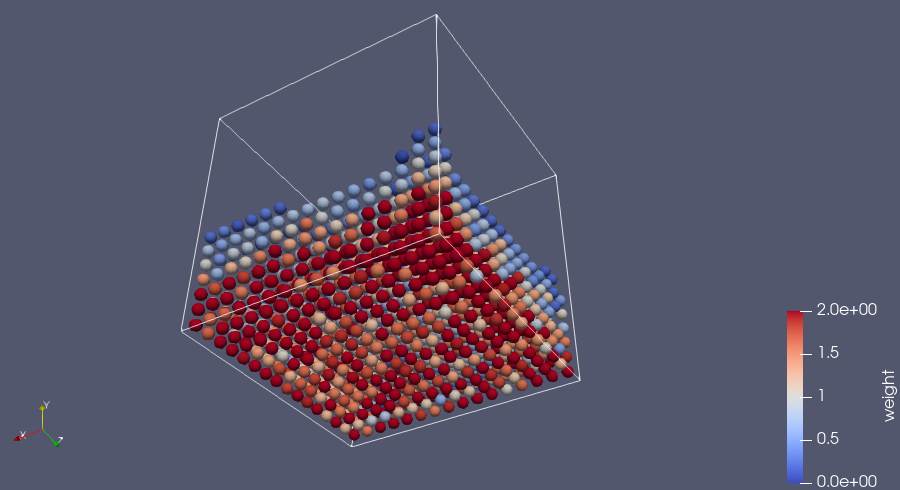
\includegraphics[width=140mm]{artificial_space.png}
\end{center}
\caption{シミュレーション領域の底面に生じた,不自然な空洞.底面から上にもある程度粒子があるのにも関わらず,周辺の粒子よりも重みが小さく,青色になっている領域があるのが見てとれる.}
\label{fig:space}
\end{figure}

\begin{figure}[H]
  \begin{minipage}[b]{0.5\linewidth}
    \centering
        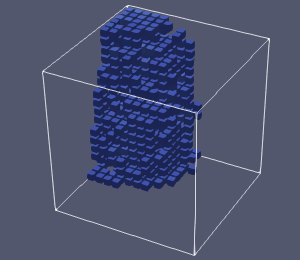
\includegraphics[width=80mm]{disipassion.png}
    \caption{格子で水の柱が拡散している様子}
    \label{fig:disipassion1}
  \end{minipage}
  \begin{minipage}[b]{0.45\linewidth}
    \centering
        \includegraphics[width=80mm]{iso_disipassion.png}
            \caption{等値面で水の柱が拡散している様子}
    \label{fig:disipassion2}
  \end{minipage}
  \begin{minipage}[b]{0.5\linewidth}
    \centering
    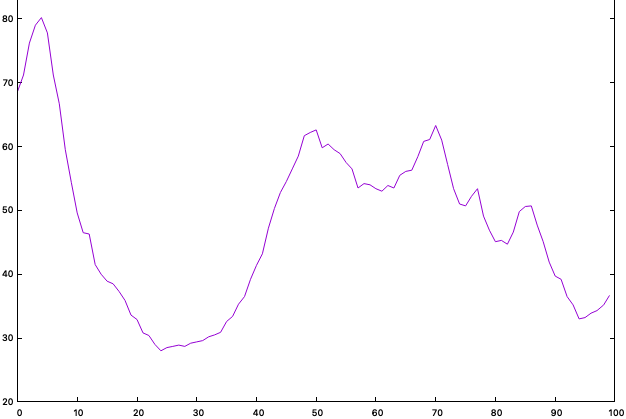
\includegraphics[width=170mm]{graph.png}
    \caption{時刻ごとの体積変化のグラフ}
     \label{fig:graph}
  \end{minipage}

\end{figure}
%%%%%%%%%%%%%%%%%%%%%
% 〇章
%%%%%%%%%%%%%%%%%%%%%
\chapter{結論} \label{chapter:6}
本研究では,流体シミュレーションの手法の一つ,FLIPでのシミュレーションに用いられる,流体の非圧縮性条件をよりよく満たすパラメータの解析を行った.流体粒子の半径や,境界面の定義に用いる閾値,粒子位置の修正の度合いを表すパラメータによって,流体の体積の変化を比較し,非圧縮性条件がより満たされているパラメータの組み合わせを解析した.
粘性のない非圧縮性流体の,ダム崩壊シミュレーションに適したパラメータとして, ($\gamma = 1.5,r = 2dx,\theta = 0.9$) , ($\gamma = 1.5,r = 2dx,\theta = 0.8$) を提案することができた.粒子半径や$\gamma$が小さいほど,粒子の密度を修正する方向に移動する距離が小さく,体積が小さくなってしまい,非圧縮条件をよく満たしているとは言えない結果が得られた,また,現実の水で働いている表面張力の影響を考慮していなかったため,水の柱が拡散しながら崩れてしまい,体積が増加してしまった.

本研究で用いたFLIPは,流体シミュレーションの基本的な手法であり,抱える問題を解決している手法が多く生み出されている.それらの手法も,体積や粘性に関する問題を抱えており,シミュレーションによって適切な手法を選択していくべきである.今後の研究では,それらの手法についての理解を深め,抱える問題点を解消する手法を提案したい.


%謝辞
\syaji
\par
本研究を進めるにあたり,研究テーマを決めるところから,研究の具体的な方針に至るまで,いつもご助言を頂いた
中央大学理工学部情報工学科の森口昌樹准教授に深く感謝いたします.論文を読む際や,研究について考えるとき,いただいたご助言によって研究をより深く理解することができました.
また,多大なるご助言,ご協力を頂いた形状情報処理研究室の同期の皆様,大学院生の皆様には大変お世話になりました.
心から感謝いたします.


%参考文献
\begin{thebibliography}{99}
\addcontentsline{toc}{chapter}{参考文献}

\bibitem{kondou}
近藤雅裕,越塚誠一,MPS法における不自然な数値振動の抑制,日本計算工学会論文集,Paper No.20080015,2008. 

\bibitem{book}
三谷純,五十嵐悠紀,岩崎慶,徳吉雄介,吉澤信,高山建志,岡部誠,向井智彦,山本醍田,辛孝宗,井尻敬,梅谷信行,安藤遼一,原田隆宏,\textit{Computer Graphics GemsJP 2012 コンピュータグラフィックス技術の最前線},株式会社 ボーンデジタル,東京都,2012.
\bibitem{PIC}
Harlow, F.H.  (1964) The Particle-in-Cell Computing Method for Fluid Dynamics. Methods in Computational Physics,\textit{Open Journal of Modelling and Simulation},  vol.4 no.~3, pp.~319--343, July 29, 2016.

\bibitem{FLIP}
J.U.Brackbill. D.B.KotheH.M.Ruppel. Flip: A low-dissipation, particle-in-cell method for fluid flow, \textit{Computer Physics Communications}, vol.48 Issue 1, pp.25--38, January 1988.

\bibitem{APIC}
K. Iwama, A. Kawachi, and S. Yamashita, The affine particle-in-cell method, IPSJ Digital Courier, \textit{ACM Transactions on Graphics}, vol. 82, Issue 4, no. 51, pp. 1--10 August 2015.
\bibitem{SPH}
Lucy, L. B. A numerical approach to the testing of the fission hypothesis, \textit{Astronomical Journal}, vol. 82, pp. 1013--1024, December. 1977.
\bibitem{MPS}
Yasutomo Kanetsuki, Susumu Nakata, Moving particle semi-implicit method for fluid simulation with implicitly defined deforming obstacles, \textit{日本シミュレーション学会英文誌}, 2巻,1号: pp.63--75, 2015.
\bibitem{MAC}
F. Losasso, F. Gibou, and R. Fedkiw. Simulating water and smoke with an octree data structure. \textit{ACM Trans. Graph.  (Proc. SIGGRAPH) }, vol. 23, pp.457--462, 2004.
\end{thebibliography}

%関連論文, 仕様はthebibliographyと同一. 
%\begin{therelatedreference}{99}
%\end{therelatedreference}
\end{document}